% Options for packages loaded elsewhere
\PassOptionsToPackage{unicode}{hyperref}
\PassOptionsToPackage{hyphens}{url}
\PassOptionsToPackage{dvipsnames,svgnames,x11names}{xcolor}
%
\documentclass[
  letterpaper,
  DIV=11,
  numbers=noendperiod]{scrartcl}

\usepackage{amsmath,amssymb}
\usepackage{iftex}
\ifPDFTeX
  \usepackage[T1]{fontenc}
  \usepackage[utf8]{inputenc}
  \usepackage{textcomp} % provide euro and other symbols
\else % if luatex or xetex
  \usepackage{unicode-math}
  \defaultfontfeatures{Scale=MatchLowercase}
  \defaultfontfeatures[\rmfamily]{Ligatures=TeX,Scale=1}
\fi
\usepackage{lmodern}
\ifPDFTeX\else  
    % xetex/luatex font selection
\fi
% Use upquote if available, for straight quotes in verbatim environments
\IfFileExists{upquote.sty}{\usepackage{upquote}}{}
\IfFileExists{microtype.sty}{% use microtype if available
  \usepackage[]{microtype}
  \UseMicrotypeSet[protrusion]{basicmath} % disable protrusion for tt fonts
}{}
\makeatletter
\@ifundefined{KOMAClassName}{% if non-KOMA class
  \IfFileExists{parskip.sty}{%
    \usepackage{parskip}
  }{% else
    \setlength{\parindent}{0pt}
    \setlength{\parskip}{6pt plus 2pt minus 1pt}}
}{% if KOMA class
  \KOMAoptions{parskip=half}}
\makeatother
\usepackage{xcolor}
\setlength{\emergencystretch}{3em} % prevent overfull lines
\setcounter{secnumdepth}{5}
% Make \paragraph and \subparagraph free-standing
\makeatletter
\ifx\paragraph\undefined\else
  \let\oldparagraph\paragraph
  \renewcommand{\paragraph}{
    \@ifstar
      \xxxParagraphStar
      \xxxParagraphNoStar
  }
  \newcommand{\xxxParagraphStar}[1]{\oldparagraph*{#1}\mbox{}}
  \newcommand{\xxxParagraphNoStar}[1]{\oldparagraph{#1}\mbox{}}
\fi
\ifx\subparagraph\undefined\else
  \let\oldsubparagraph\subparagraph
  \renewcommand{\subparagraph}{
    \@ifstar
      \xxxSubParagraphStar
      \xxxSubParagraphNoStar
  }
  \newcommand{\xxxSubParagraphStar}[1]{\oldsubparagraph*{#1}\mbox{}}
  \newcommand{\xxxSubParagraphNoStar}[1]{\oldsubparagraph{#1}\mbox{}}
\fi
\makeatother

\usepackage{color}
\usepackage{fancyvrb}
\newcommand{\VerbBar}{|}
\newcommand{\VERB}{\Verb[commandchars=\\\{\}]}
\DefineVerbatimEnvironment{Highlighting}{Verbatim}{commandchars=\\\{\}}
% Add ',fontsize=\small' for more characters per line
\usepackage{framed}
\definecolor{shadecolor}{RGB}{241,243,245}
\newenvironment{Shaded}{\begin{snugshade}}{\end{snugshade}}
\newcommand{\AlertTok}[1]{\textcolor[rgb]{0.68,0.00,0.00}{#1}}
\newcommand{\AnnotationTok}[1]{\textcolor[rgb]{0.37,0.37,0.37}{#1}}
\newcommand{\AttributeTok}[1]{\textcolor[rgb]{0.40,0.45,0.13}{#1}}
\newcommand{\BaseNTok}[1]{\textcolor[rgb]{0.68,0.00,0.00}{#1}}
\newcommand{\BuiltInTok}[1]{\textcolor[rgb]{0.00,0.23,0.31}{#1}}
\newcommand{\CharTok}[1]{\textcolor[rgb]{0.13,0.47,0.30}{#1}}
\newcommand{\CommentTok}[1]{\textcolor[rgb]{0.37,0.37,0.37}{#1}}
\newcommand{\CommentVarTok}[1]{\textcolor[rgb]{0.37,0.37,0.37}{\textit{#1}}}
\newcommand{\ConstantTok}[1]{\textcolor[rgb]{0.56,0.35,0.01}{#1}}
\newcommand{\ControlFlowTok}[1]{\textcolor[rgb]{0.00,0.23,0.31}{\textbf{#1}}}
\newcommand{\DataTypeTok}[1]{\textcolor[rgb]{0.68,0.00,0.00}{#1}}
\newcommand{\DecValTok}[1]{\textcolor[rgb]{0.68,0.00,0.00}{#1}}
\newcommand{\DocumentationTok}[1]{\textcolor[rgb]{0.37,0.37,0.37}{\textit{#1}}}
\newcommand{\ErrorTok}[1]{\textcolor[rgb]{0.68,0.00,0.00}{#1}}
\newcommand{\ExtensionTok}[1]{\textcolor[rgb]{0.00,0.23,0.31}{#1}}
\newcommand{\FloatTok}[1]{\textcolor[rgb]{0.68,0.00,0.00}{#1}}
\newcommand{\FunctionTok}[1]{\textcolor[rgb]{0.28,0.35,0.67}{#1}}
\newcommand{\ImportTok}[1]{\textcolor[rgb]{0.00,0.46,0.62}{#1}}
\newcommand{\InformationTok}[1]{\textcolor[rgb]{0.37,0.37,0.37}{#1}}
\newcommand{\KeywordTok}[1]{\textcolor[rgb]{0.00,0.23,0.31}{\textbf{#1}}}
\newcommand{\NormalTok}[1]{\textcolor[rgb]{0.00,0.23,0.31}{#1}}
\newcommand{\OperatorTok}[1]{\textcolor[rgb]{0.37,0.37,0.37}{#1}}
\newcommand{\OtherTok}[1]{\textcolor[rgb]{0.00,0.23,0.31}{#1}}
\newcommand{\PreprocessorTok}[1]{\textcolor[rgb]{0.68,0.00,0.00}{#1}}
\newcommand{\RegionMarkerTok}[1]{\textcolor[rgb]{0.00,0.23,0.31}{#1}}
\newcommand{\SpecialCharTok}[1]{\textcolor[rgb]{0.37,0.37,0.37}{#1}}
\newcommand{\SpecialStringTok}[1]{\textcolor[rgb]{0.13,0.47,0.30}{#1}}
\newcommand{\StringTok}[1]{\textcolor[rgb]{0.13,0.47,0.30}{#1}}
\newcommand{\VariableTok}[1]{\textcolor[rgb]{0.07,0.07,0.07}{#1}}
\newcommand{\VerbatimStringTok}[1]{\textcolor[rgb]{0.13,0.47,0.30}{#1}}
\newcommand{\WarningTok}[1]{\textcolor[rgb]{0.37,0.37,0.37}{\textit{#1}}}

\providecommand{\tightlist}{%
  \setlength{\itemsep}{0pt}\setlength{\parskip}{0pt}}\usepackage{longtable,booktabs,array}
\usepackage{calc} % for calculating minipage widths
% Correct order of tables after \paragraph or \subparagraph
\usepackage{etoolbox}
\makeatletter
\patchcmd\longtable{\par}{\if@noskipsec\mbox{}\fi\par}{}{}
\makeatother
% Allow footnotes in longtable head/foot
\IfFileExists{footnotehyper.sty}{\usepackage{footnotehyper}}{\usepackage{footnote}}
\makesavenoteenv{longtable}
\usepackage{graphicx}
\makeatletter
\newsavebox\pandoc@box
\newcommand*\pandocbounded[1]{% scales image to fit in text height/width
  \sbox\pandoc@box{#1}%
  \Gscale@div\@tempa{\textheight}{\dimexpr\ht\pandoc@box+\dp\pandoc@box\relax}%
  \Gscale@div\@tempb{\linewidth}{\wd\pandoc@box}%
  \ifdim\@tempb\p@<\@tempa\p@\let\@tempa\@tempb\fi% select the smaller of both
  \ifdim\@tempa\p@<\p@\scalebox{\@tempa}{\usebox\pandoc@box}%
  \else\usebox{\pandoc@box}%
  \fi%
}
% Set default figure placement to htbp
\def\fps@figure{htbp}
\makeatother

\KOMAoption{captions}{tableheading,figureheading}
\makeatletter
\@ifpackageloaded{caption}{}{\usepackage{caption}}
\AtBeginDocument{%
\ifdefined\contentsname
  \renewcommand*\contentsname{Table of contents}
\else
  \newcommand\contentsname{Table of contents}
\fi
\ifdefined\listfigurename
  \renewcommand*\listfigurename{List of Figures}
\else
  \newcommand\listfigurename{List of Figures}
\fi
\ifdefined\listtablename
  \renewcommand*\listtablename{List of Tables}
\else
  \newcommand\listtablename{List of Tables}
\fi
\ifdefined\figurename
  \renewcommand*\figurename{Figure}
\else
  \newcommand\figurename{Figure}
\fi
\ifdefined\tablename
  \renewcommand*\tablename{Table}
\else
  \newcommand\tablename{Table}
\fi
}
\@ifpackageloaded{float}{}{\usepackage{float}}
\floatstyle{ruled}
\@ifundefined{c@chapter}{\newfloat{codelisting}{h}{lop}}{\newfloat{codelisting}{h}{lop}[chapter]}
\floatname{codelisting}{Listing}
\newcommand*\listoflistings{\listof{codelisting}{List of Listings}}
\makeatother
\makeatletter
\makeatother
\makeatletter
\@ifpackageloaded{caption}{}{\usepackage{caption}}
\@ifpackageloaded{subcaption}{}{\usepackage{subcaption}}
\makeatother

\usepackage{bookmark}

\IfFileExists{xurl.sty}{\usepackage{xurl}}{} % add URL line breaks if available
\urlstyle{same} % disable monospaced font for URLs
\hypersetup{
  pdftitle={Introduction to Python},
  pdfauthor={Sandro Ricardo De Souza},
  colorlinks=true,
  linkcolor={blue},
  filecolor={Maroon},
  citecolor={Blue},
  urlcolor={Blue},
  pdfcreator={LaTeX via pandoc}}


\title{Introduction to Python}
\author{Sandro Ricardo De Souza}
\date{2024-07-01}

\begin{document}
\maketitle

\renewcommand*\contentsname{Table of contents}
{
\hypersetup{linkcolor=}
\setcounter{tocdepth}{2}
\tableofcontents
}

\section{Identificação de Perfis de Estudantes com Modelos
Descritivos}\label{identificauxe7uxe3o-de-perfis-de-estudantes-com-modelos-descritivos}

\subsection{Parte 1: Conteúdo Teórico
Explicativo}\label{parte-1-conteuxfado-teuxf3rico-explicativo}

Este notebook tem como objetivo demonstrar a identificação de perfis de
estudantes com base em dados educacionais, utilizando modelos
descritivos e técnicas de agrupamento (clustering).

Pontos-chave: - Modelos descritivos ajudam a resumir, explorar e
visualizar dados. - No contexto educacional, podemos usar esses modelos
para identificar perfis de engajamento e desempenho. - O clustering é
uma técnica não supervisionada que agrupa instâncias semelhantes entre
si.

Técnicas usadas neste notebook: - Estatística descritiva (média, desvio
padrão) - Visualização de dados (gráficos) - K-means clustering

\subsection{Parte 2: Exemplo Prático}\label{parte-2-exemplo-pruxe1tico}

\subsection{Importação de
Bibliotecas}\label{importauxe7uxe3o-de-bibliotecas}

\begin{Shaded}
\begin{Highlighting}[]
\ImportTok{import}\NormalTok{ pandas }\ImportTok{as}\NormalTok{ pd}
\ImportTok{import}\NormalTok{ numpy }\ImportTok{as}\NormalTok{ np}
\ImportTok{import}\NormalTok{ matplotlib.pyplot }\ImportTok{as}\NormalTok{ plt}
\ImportTok{import}\NormalTok{ seaborn }\ImportTok{as}\NormalTok{ sns}
\ImportTok{from}\NormalTok{ sklearn.cluster }\ImportTok{import}\NormalTok{ KMeans}
\ImportTok{from}\NormalTok{ sklearn.preprocessing }\ImportTok{import}\NormalTok{ StandardScaler}
\ImportTok{from}\NormalTok{ sklearn.decomposition }\ImportTok{import}\NormalTok{ PCA}
\ImportTok{from}\NormalTok{ sklearn.metrics }\ImportTok{import}\NormalTok{ silhouette\_score}
\end{Highlighting}
\end{Shaded}

\subsection{Carregamento do Dataset
Exemplo}\label{carregamento-do-dataset-exemplo}

O dataset simulado contém dados de estudantes com as seguintes colunas:
- `id': identificador do estudante - `acessos': número de acessos ao AVA
- `participacoes': número de interações em fóruns - `entregas':
percentual de tarefas entregues - `nota\_final': nota final no curso

\begin{Shaded}
\begin{Highlighting}[]
\CommentTok{\# Dataset simulado}

\NormalTok{data }\OperatorTok{=}\NormalTok{ \{}
    \StringTok{\textquotesingle{}id\textquotesingle{}}\NormalTok{: }\BuiltInTok{range}\NormalTok{(}\DecValTok{1}\NormalTok{, }\DecValTok{21}\NormalTok{),}
    \StringTok{\textquotesingle{}acessos\textquotesingle{}}\NormalTok{: [}\DecValTok{25}\NormalTok{, }\DecValTok{10}\NormalTok{, }\DecValTok{5}\NormalTok{, }\DecValTok{40}\NormalTok{, }\DecValTok{35}\NormalTok{, }\DecValTok{20}\NormalTok{, }\DecValTok{15}\NormalTok{, }\DecValTok{8}\NormalTok{, }\DecValTok{50}\NormalTok{, }\DecValTok{30}\NormalTok{, }\DecValTok{45}\NormalTok{, }\DecValTok{12}\NormalTok{, }\DecValTok{18}\NormalTok{, }\DecValTok{22}\NormalTok{, }\DecValTok{28}\NormalTok{, }\DecValTok{6}\NormalTok{, }\DecValTok{4}\NormalTok{, }\DecValTok{38}\NormalTok{, }\DecValTok{44}\NormalTok{, }\DecValTok{7}\NormalTok{],}
    \StringTok{\textquotesingle{}participacoes\textquotesingle{}}\NormalTok{: [}\DecValTok{12}\NormalTok{, }\DecValTok{4}\NormalTok{, }\DecValTok{2}\NormalTok{, }\DecValTok{18}\NormalTok{, }\DecValTok{16}\NormalTok{, }\DecValTok{8}\NormalTok{, }\DecValTok{5}\NormalTok{, }\DecValTok{2}\NormalTok{, }\DecValTok{20}\NormalTok{, }\DecValTok{14}\NormalTok{, }\DecValTok{19}\NormalTok{, }\DecValTok{3}\NormalTok{, }\DecValTok{6}\NormalTok{, }\DecValTok{10}\NormalTok{, }\DecValTok{11}\NormalTok{, }\DecValTok{1}\NormalTok{, }\DecValTok{0}\NormalTok{, }\DecValTok{17}\NormalTok{, }\DecValTok{18}\NormalTok{, }\DecValTok{2}\NormalTok{],}
    \StringTok{\textquotesingle{}entregas\textquotesingle{}}\NormalTok{: [}\FloatTok{0.9}\NormalTok{, }\FloatTok{0.6}\NormalTok{, }\FloatTok{0.4}\NormalTok{, }\FloatTok{1.0}\NormalTok{, }\FloatTok{0.95}\NormalTok{, }\FloatTok{0.8}\NormalTok{, }\FloatTok{0.7}\NormalTok{, }\FloatTok{0.5}\NormalTok{, }\FloatTok{1.0}\NormalTok{, }\FloatTok{0.85}\NormalTok{, }\FloatTok{1.0}\NormalTok{, }\FloatTok{0.55}\NormalTok{, }\FloatTok{0.65}\NormalTok{, }\FloatTok{0.75}\NormalTok{, }\FloatTok{0.8}\NormalTok{, }\FloatTok{0.3}\NormalTok{, }\FloatTok{0.2}\NormalTok{, }\FloatTok{0.9}\NormalTok{, }\FloatTok{1.0}\NormalTok{, }\FloatTok{0.4}\NormalTok{],}
    \StringTok{\textquotesingle{}nota\_final\textquotesingle{}}\NormalTok{: [}\FloatTok{8.5}\NormalTok{, }\FloatTok{6.0}\NormalTok{, }\FloatTok{4.5}\NormalTok{, }\FloatTok{9.5}\NormalTok{, }\FloatTok{9.0}\NormalTok{, }\FloatTok{7.5}\NormalTok{, }\FloatTok{6.5}\NormalTok{, }\FloatTok{5.0}\NormalTok{, }\FloatTok{10.0}\NormalTok{, }\FloatTok{8.0}\NormalTok{, }\FloatTok{9.5}\NormalTok{, }\FloatTok{5.5}\NormalTok{, }\FloatTok{6.0}\NormalTok{, }\FloatTok{7.0}\NormalTok{, }\FloatTok{7.5}\NormalTok{, }\FloatTok{3.5}\NormalTok{, }\FloatTok{2.0}\NormalTok{, }\FloatTok{8.5}\NormalTok{, }\FloatTok{9.5}\NormalTok{, }\FloatTok{4.0}\NormalTok{]}
\NormalTok{\}}
\NormalTok{df }\OperatorTok{=}\NormalTok{ pd.DataFrame(data)}
\NormalTok{df.head()}
\end{Highlighting}
\end{Shaded}

\begin{longtable}[]{@{}llllll@{}}
\toprule\noalign{}
& id & acessos & participacoes & entregas & nota\_final \\
\midrule\noalign{}
\endhead
\bottomrule\noalign{}
\endlastfoot
0 & 1 & 25 & 12 & 0.90 & 8.5 \\
1 & 2 & 10 & 4 & 0.60 & 6.0 \\
2 & 3 & 5 & 2 & 0.40 & 4.5 \\
3 & 4 & 40 & 18 & 1.00 & 9.5 \\
4 & 5 & 35 & 16 & 0.95 & 9.0 \\
\end{longtable}

\subsubsection{Estatística Descritiva}\label{estatuxedstica-descritiva}

\begin{Shaded}
\begin{Highlighting}[]
\BuiltInTok{print}\NormalTok{(}\StringTok{"}\CharTok{\textbackslash{}n}\StringTok{Estatísticas Descritivas:"}\NormalTok{)}
\NormalTok{df.describe()}
\end{Highlighting}
\end{Shaded}

\begin{verbatim}

Estatísticas Descritivas:
\end{verbatim}

\begin{longtable}[]{@{}llllll@{}}
\toprule\noalign{}
& id & acessos & participacoes & entregas & nota\_final \\
\midrule\noalign{}
\endhead
\bottomrule\noalign{}
\endlastfoot
count & 20.00000 & 20.000000 & 20.000000 & 20.000000 & 20.000000 \\
mean & 10.50000 & 23.100000 & 9.400000 & 0.712500 & 6.875000 \\
std & 5.91608 & 14.927544 & 6.923644 & 0.252292 & 2.276164 \\
min & 1.00000 & 4.000000 & 0.000000 & 0.200000 & 2.000000 \\
25\% & 5.75000 & 9.500000 & 2.750000 & 0.537500 & 5.375000 \\
50\% & 10.50000 & 21.000000 & 9.000000 & 0.775000 & 7.250000 \\
75\% & 15.25000 & 35.750000 & 16.250000 & 0.912500 & 8.625000 \\
max & 20.00000 & 50.000000 & 20.000000 & 1.000000 & 10.000000 \\
\end{longtable}

\subsubsection{Visualização Inicial dos
Dados}\label{visualizauxe7uxe3o-inicial-dos-dados}

\begin{Shaded}
\begin{Highlighting}[]
\NormalTok{sns.pairplot(df.drop(}\StringTok{\textquotesingle{}id\textquotesingle{}}\NormalTok{, axis}\OperatorTok{=}\DecValTok{1}\NormalTok{))}
\NormalTok{plt.suptitle(}\StringTok{\textquotesingle{}Visualização Inicial das Variáveis\textquotesingle{}}\NormalTok{, y}\OperatorTok{=}\FloatTok{1.02}\NormalTok{)}
\NormalTok{plt.show()}
\end{Highlighting}
\end{Shaded}

\pandocbounded{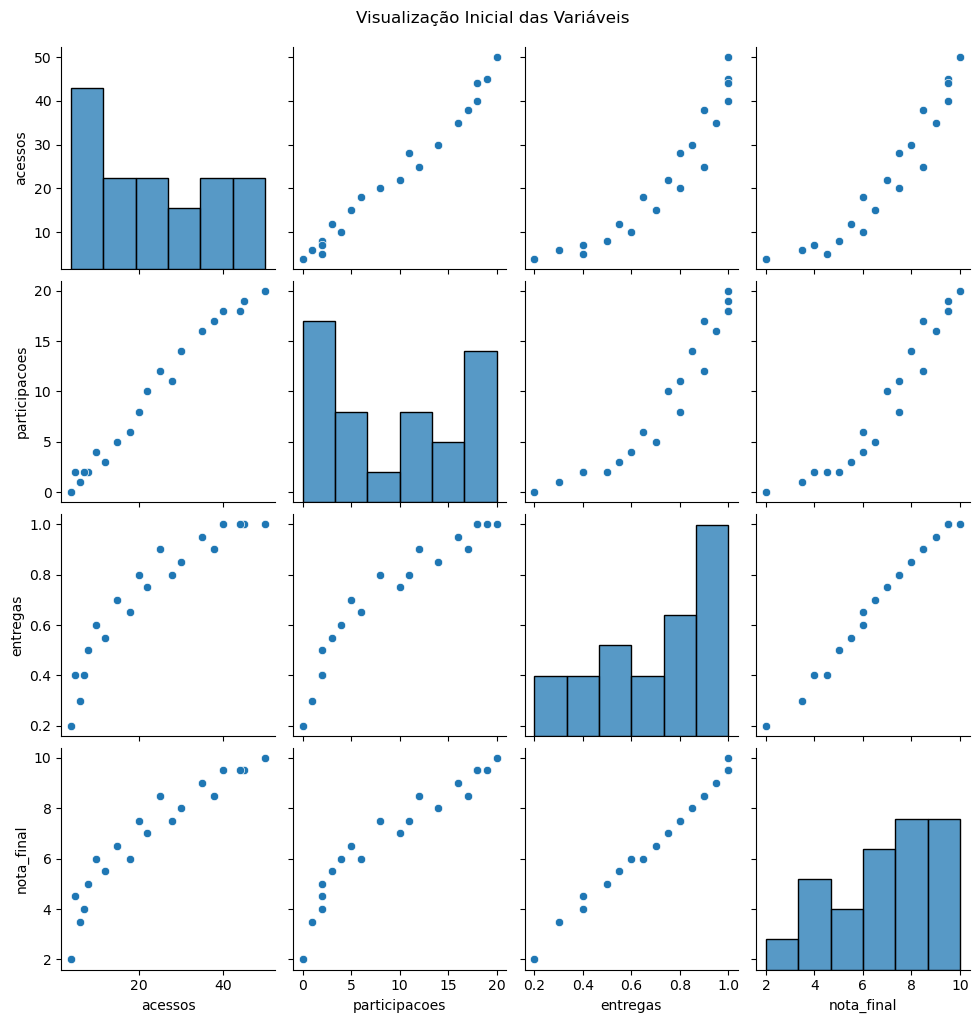
\includegraphics[keepaspectratio]{teste_quarto_files/figure-pdf/cell-5-output-1.png}}

\subsubsection{Normalização dos
Dados}\label{normalizauxe7uxe3o-dos-dados}

\begin{Shaded}
\begin{Highlighting}[]
\NormalTok{features }\OperatorTok{=}\NormalTok{ [}\StringTok{\textquotesingle{}acessos\textquotesingle{}}\NormalTok{, }\StringTok{\textquotesingle{}participacoes\textquotesingle{}}\NormalTok{, }\StringTok{\textquotesingle{}entregas\textquotesingle{}}\NormalTok{, }\StringTok{\textquotesingle{}nota\_final\textquotesingle{}}\NormalTok{]}
\NormalTok{scaler }\OperatorTok{=}\NormalTok{ StandardScaler()}
\NormalTok{df\_scaled }\OperatorTok{=}\NormalTok{ scaler.fit\_transform(df[features])}
\end{Highlighting}
\end{Shaded}

\subsubsection{Determinação do Melhor Número de Clusters com
Silhouette}\label{determinauxe7uxe3o-do-melhor-nuxfamero-de-clusters-com-silhouette}

\begin{Shaded}
\begin{Highlighting}[]
\NormalTok{range\_n\_clusters }\OperatorTok{=} \BuiltInTok{range}\NormalTok{(}\DecValTok{2}\NormalTok{, }\DecValTok{10}\NormalTok{)}
\NormalTok{best\_n }\OperatorTok{=} \DecValTok{2}
\NormalTok{best\_score }\OperatorTok{=} \OperatorTok{{-}}\DecValTok{1}

\ControlFlowTok{for}\NormalTok{ n\_clusters }\KeywordTok{in}\NormalTok{ range\_n\_clusters:}
\NormalTok{    kmeans }\OperatorTok{=}\NormalTok{ KMeans(n\_clusters}\OperatorTok{=}\NormalTok{n\_clusters, random\_state}\OperatorTok{=}\DecValTok{42}\NormalTok{)}
\NormalTok{    cluster\_labels }\OperatorTok{=}\NormalTok{ kmeans.fit\_predict(df\_scaled)}
\NormalTok{    silhouette\_avg }\OperatorTok{=}\NormalTok{ silhouette\_score(df\_scaled, cluster\_labels)}
    \BuiltInTok{print}\NormalTok{(}\SpecialStringTok{f"Para n\_clusters = }\SpecialCharTok{\{}\NormalTok{n\_clusters}\SpecialCharTok{\}}\SpecialStringTok{, o coeficiente de silhouette é }\SpecialCharTok{\{}\NormalTok{silhouette\_avg}\SpecialCharTok{:.4f\}}\SpecialStringTok{"}\NormalTok{)}
    \ControlFlowTok{if}\NormalTok{ silhouette\_avg }\OperatorTok{\textgreater{}}\NormalTok{ best\_score:}
\NormalTok{        best\_n }\OperatorTok{=}\NormalTok{ n\_clusters}
\NormalTok{        best\_score }\OperatorTok{=}\NormalTok{ silhouette\_avg}

\BuiltInTok{print}\NormalTok{(}\SpecialStringTok{f"}\CharTok{\textbackslash{}n}\SpecialStringTok{Melhor número de clusters com base no silhouette: }\SpecialCharTok{\{}\NormalTok{best\_n}\SpecialCharTok{\}}\SpecialStringTok{"}\NormalTok{)}
\end{Highlighting}
\end{Shaded}

\begin{verbatim}
Para n_clusters = 2, o coeficiente de silhouette é 0.5704
Para n_clusters = 3, o coeficiente de silhouette é 0.5292
Para n_clusters = 4, o coeficiente de silhouette é 0.4198
Para n_clusters = 5, o coeficiente de silhouette é 0.3869
Para n_clusters = 6, o coeficiente de silhouette é 0.3555
Para n_clusters = 7, o coeficiente de silhouette é 0.3754
Para n_clusters = 8, o coeficiente de silhouette é 0.2681
Para n_clusters = 9, o coeficiente de silhouette é 0.2372

Melhor número de clusters com base no silhouette: 2
\end{verbatim}

\begin{verbatim}
c:\Users\srsouza\AppData\Local\anaconda3\Lib\site-packages\sklearn\cluster\_kmeans.py:1429: UserWarning: KMeans is known to have a memory leak on Windows with MKL, when there are less chunks than available threads. You can avoid it by setting the environment variable OMP_NUM_THREADS=1.
  warnings.warn(
c:\Users\srsouza\AppData\Local\anaconda3\Lib\site-packages\sklearn\cluster\_kmeans.py:1429: UserWarning: KMeans is known to have a memory leak on Windows with MKL, when there are less chunks than available threads. You can avoid it by setting the environment variable OMP_NUM_THREADS=1.
  warnings.warn(
c:\Users\srsouza\AppData\Local\anaconda3\Lib\site-packages\sklearn\cluster\_kmeans.py:1429: UserWarning: KMeans is known to have a memory leak on Windows with MKL, when there are less chunks than available threads. You can avoid it by setting the environment variable OMP_NUM_THREADS=1.
  warnings.warn(
c:\Users\srsouza\AppData\Local\anaconda3\Lib\site-packages\sklearn\cluster\_kmeans.py:1429: UserWarning: KMeans is known to have a memory leak on Windows with MKL, when there are less chunks than available threads. You can avoid it by setting the environment variable OMP_NUM_THREADS=1.
  warnings.warn(
c:\Users\srsouza\AppData\Local\anaconda3\Lib\site-packages\sklearn\cluster\_kmeans.py:1429: UserWarning: KMeans is known to have a memory leak on Windows with MKL, when there are less chunks than available threads. You can avoid it by setting the environment variable OMP_NUM_THREADS=1.
  warnings.warn(
c:\Users\srsouza\AppData\Local\anaconda3\Lib\site-packages\sklearn\cluster\_kmeans.py:1429: UserWarning: KMeans is known to have a memory leak on Windows with MKL, when there are less chunks than available threads. You can avoid it by setting the environment variable OMP_NUM_THREADS=1.
  warnings.warn(
c:\Users\srsouza\AppData\Local\anaconda3\Lib\site-packages\sklearn\cluster\_kmeans.py:1429: UserWarning: KMeans is known to have a memory leak on Windows with MKL, when there are less chunks than available threads. You can avoid it by setting the environment variable OMP_NUM_THREADS=1.
  warnings.warn(
c:\Users\srsouza\AppData\Local\anaconda3\Lib\site-packages\sklearn\cluster\_kmeans.py:1429: UserWarning: KMeans is known to have a memory leak on Windows with MKL, when there are less chunks than available threads. You can avoid it by setting the environment variable OMP_NUM_THREADS=1.
  warnings.warn(
\end{verbatim}

\subsubsection{Aplicando KMeans com o melhor número de
clusters}\label{aplicando-kmeans-com-o-melhor-nuxfamero-de-clusters}

\begin{Shaded}
\begin{Highlighting}[]
\NormalTok{kmeans }\OperatorTok{=}\NormalTok{ KMeans(n\_clusters}\OperatorTok{=}\NormalTok{best\_n, random\_state}\OperatorTok{=}\DecValTok{42}\NormalTok{)}
\NormalTok{df[}\StringTok{\textquotesingle{}cluster\textquotesingle{}}\NormalTok{] }\OperatorTok{=}\NormalTok{ kmeans.fit\_predict(df\_scaled)}
\end{Highlighting}
\end{Shaded}

\begin{verbatim}
c:\Users\srsouza\AppData\Local\anaconda3\Lib\site-packages\sklearn\cluster\_kmeans.py:1429: UserWarning: KMeans is known to have a memory leak on Windows with MKL, when there are less chunks than available threads. You can avoid it by setting the environment variable OMP_NUM_THREADS=1.
  warnings.warn(
\end{verbatim}

\begin{Shaded}
\begin{Highlighting}[]
\NormalTok{df}
\end{Highlighting}
\end{Shaded}

\begin{longtable}[]{@{}lllllll@{}}
\toprule\noalign{}
& id & acessos & participacoes & entregas & nota\_final & cluster \\
\midrule\noalign{}
\endhead
\bottomrule\noalign{}
\endlastfoot
0 & 1 & 25 & 12 & 0.90 & 8.5 & 1 \\
1 & 2 & 10 & 4 & 0.60 & 6.0 & 0 \\
2 & 3 & 5 & 2 & 0.40 & 4.5 & 0 \\
3 & 4 & 40 & 18 & 1.00 & 9.5 & 1 \\
4 & 5 & 35 & 16 & 0.95 & 9.0 & 1 \\
5 & 6 & 20 & 8 & 0.80 & 7.5 & 0 \\
6 & 7 & 15 & 5 & 0.70 & 6.5 & 0 \\
7 & 8 & 8 & 2 & 0.50 & 5.0 & 0 \\
8 & 9 & 50 & 20 & 1.00 & 10.0 & 1 \\
9 & 10 & 30 & 14 & 0.85 & 8.0 & 1 \\
10 & 11 & 45 & 19 & 1.00 & 9.5 & 1 \\
11 & 12 & 12 & 3 & 0.55 & 5.5 & 0 \\
12 & 13 & 18 & 6 & 0.65 & 6.0 & 0 \\
13 & 14 & 22 & 10 & 0.75 & 7.0 & 0 \\
14 & 15 & 28 & 11 & 0.80 & 7.5 & 1 \\
15 & 16 & 6 & 1 & 0.30 & 3.5 & 0 \\
16 & 17 & 4 & 0 & 0.20 & 2.0 & 0 \\
17 & 18 & 38 & 17 & 0.90 & 8.5 & 1 \\
18 & 19 & 44 & 18 & 1.00 & 9.5 & 1 \\
19 & 20 & 7 & 2 & 0.40 & 4.0 & 0 \\
\end{longtable}

\subsubsection{Analise os grupos 0 e 1 e informe as característica de
cada
grupo.}\label{analise-os-grupos-0-e-1-e-informe-as-caracteruxedstica-de-cada-grupo.}

\begin{Shaded}
\begin{Highlighting}[]
\NormalTok{df}
\end{Highlighting}
\end{Shaded}

\begin{longtable}[]{@{}lllllll@{}}
\toprule\noalign{}
& id & acessos & participacoes & entregas & nota\_final & cluster \\
\midrule\noalign{}
\endhead
\bottomrule\noalign{}
\endlastfoot
0 & 1 & 25 & 12 & 0.90 & 8.5 & 1 \\
1 & 2 & 10 & 4 & 0.60 & 6.0 & 0 \\
2 & 3 & 5 & 2 & 0.40 & 4.5 & 0 \\
3 & 4 & 40 & 18 & 1.00 & 9.5 & 1 \\
4 & 5 & 35 & 16 & 0.95 & 9.0 & 1 \\
5 & 6 & 20 & 8 & 0.80 & 7.5 & 0 \\
6 & 7 & 15 & 5 & 0.70 & 6.5 & 0 \\
7 & 8 & 8 & 2 & 0.50 & 5.0 & 0 \\
8 & 9 & 50 & 20 & 1.00 & 10.0 & 1 \\
9 & 10 & 30 & 14 & 0.85 & 8.0 & 1 \\
10 & 11 & 45 & 19 & 1.00 & 9.5 & 1 \\
11 & 12 & 12 & 3 & 0.55 & 5.5 & 0 \\
12 & 13 & 18 & 6 & 0.65 & 6.0 & 0 \\
13 & 14 & 22 & 10 & 0.75 & 7.0 & 0 \\
14 & 15 & 28 & 11 & 0.80 & 7.5 & 1 \\
15 & 16 & 6 & 1 & 0.30 & 3.5 & 0 \\
16 & 17 & 4 & 0 & 0.20 & 2.0 & 0 \\
17 & 18 & 38 & 17 & 0.90 & 8.5 & 1 \\
18 & 19 & 44 & 18 & 1.00 & 9.5 & 1 \\
19 & 20 & 7 & 2 & 0.40 & 4.0 & 0 \\
\end{longtable}

\begin{Shaded}
\begin{Highlighting}[]
\NormalTok{summary }\OperatorTok{=}\NormalTok{ \{\}}

\NormalTok{Labels }\OperatorTok{=}\NormalTok{ [}\StringTok{\textquotesingle{}acessos\textquotesingle{}}\NormalTok{, }\StringTok{\textquotesingle{}participacoes\textquotesingle{}}\NormalTok{, }\StringTok{\textquotesingle{}entregas\textquotesingle{}}\NormalTok{, }\StringTok{\textquotesingle{}nota\_final\textquotesingle{}}\NormalTok{]}

\ControlFlowTok{for}\NormalTok{ label }\KeywordTok{in}\NormalTok{ Labels:}
    \ControlFlowTok{for}\NormalTok{ index }\KeywordTok{in} \BuiltInTok{range}\NormalTok{(}\DecValTok{2}\NormalTok{):}
\NormalTok{        summary[index] }\OperatorTok{=}\NormalTok{ df[df[label] }\OperatorTok{==}\NormalTok{ index].describe().T  }\CommentTok{\# .describe method provides general statistics about the data}
\end{Highlighting}
\end{Shaded}

\begin{Shaded}
\begin{Highlighting}[]
\NormalTok{summary[}\DecValTok{0}\NormalTok{]}
\end{Highlighting}
\end{Shaded}

\begin{longtable}[]{@{}lllllllll@{}}
\toprule\noalign{}
& count & mean & std & min & 25\% & 50\% & 75\% & max \\
\midrule\noalign{}
\endhead
\bottomrule\noalign{}
\endlastfoot
id & 0.0 & NaN & NaN & NaN & NaN & NaN & NaN & NaN \\
acessos & 0.0 & NaN & NaN & NaN & NaN & NaN & NaN & NaN \\
participacoes & 0.0 & NaN & NaN & NaN & NaN & NaN & NaN & NaN \\
entregas & 0.0 & NaN & NaN & NaN & NaN & NaN & NaN & NaN \\
nota\_final & 0.0 & NaN & NaN & NaN & NaN & NaN & NaN & NaN \\
cluster & 0.0 & NaN & NaN & NaN & NaN & NaN & NaN & NaN \\
\end{longtable}

\begin{Shaded}
\begin{Highlighting}[]
\CommentTok{\# GRUPO 0: Coloque seu código aqui...}

\NormalTok{df[df[}\StringTok{\textquotesingle{}cluster\textquotesingle{}}\NormalTok{] }\OperatorTok{==} \DecValTok{0}\NormalTok{].hist(figsize}\OperatorTok{=}\NormalTok{(}\DecValTok{10}\NormalTok{,}\DecValTok{10}\NormalTok{))}\OperatorTok{;}
\end{Highlighting}
\end{Shaded}

\pandocbounded{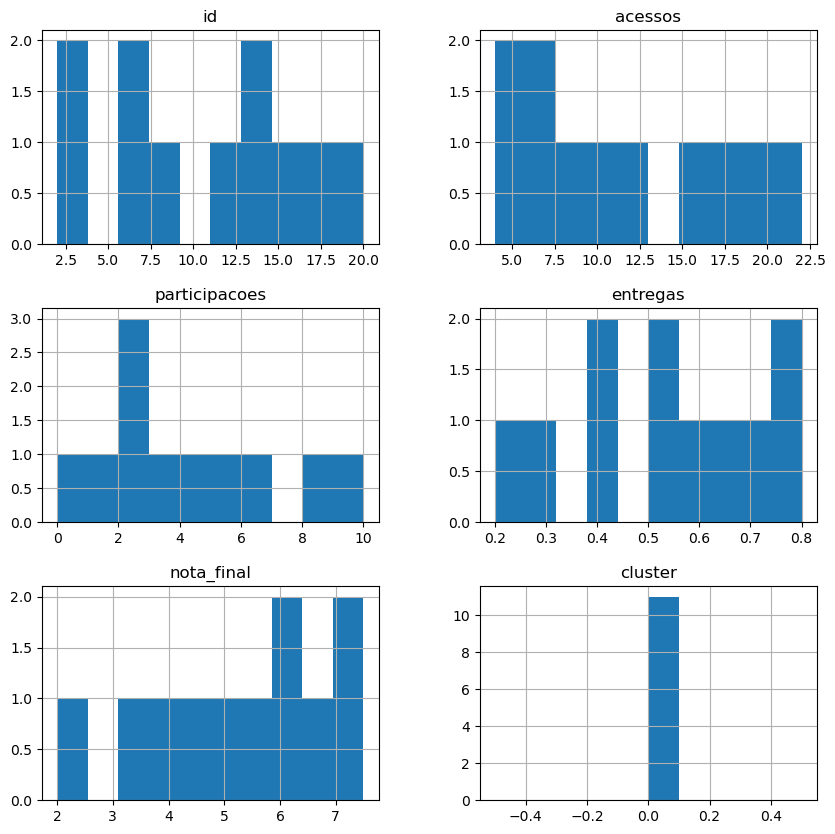
\includegraphics[keepaspectratio]{teste_quarto_files/figure-pdf/cell-13-output-1.png}}

\begin{Shaded}
\begin{Highlighting}[]
\CommentTok{\# GRUPO 1: Coloque seu código aqui...}
\NormalTok{df[df[}\StringTok{\textquotesingle{}cluster\textquotesingle{}}\NormalTok{] }\OperatorTok{==} \DecValTok{1}\NormalTok{].hist(figsize}\OperatorTok{=}\NormalTok{(}\DecValTok{10}\NormalTok{,}\DecValTok{10}\NormalTok{))}\OperatorTok{;}
\end{Highlighting}
\end{Shaded}

\pandocbounded{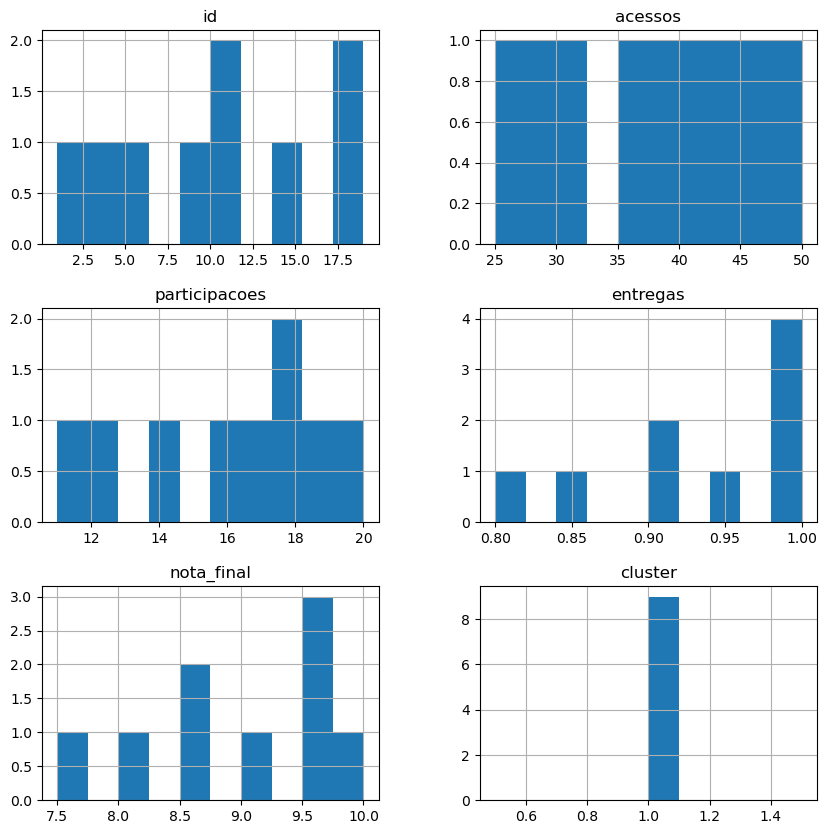
\includegraphics[keepaspectratio]{teste_quarto_files/figure-pdf/cell-14-output-1.png}}

\subsubsection{Visualização dos Clusters com
PCA}\label{visualizauxe7uxe3o-dos-clusters-com-pca}

\begin{Shaded}
\begin{Highlighting}[]
\NormalTok{pca }\OperatorTok{=}\NormalTok{ PCA(n\_components}\OperatorTok{=}\DecValTok{2}\NormalTok{)}
\NormalTok{df\_pca }\OperatorTok{=}\NormalTok{ pca.fit\_transform(df\_scaled)}
\NormalTok{df[}\StringTok{\textquotesingle{}pca1\textquotesingle{}}\NormalTok{] }\OperatorTok{=}\NormalTok{ df\_pca[:, }\DecValTok{0}\NormalTok{]}
\NormalTok{df[}\StringTok{\textquotesingle{}pca2\textquotesingle{}}\NormalTok{] }\OperatorTok{=}\NormalTok{ df\_pca[:, }\DecValTok{1}\NormalTok{]}

\NormalTok{plt.figure(figsize}\OperatorTok{=}\NormalTok{(}\DecValTok{8}\NormalTok{,}\DecValTok{6}\NormalTok{))}
\NormalTok{sns.scatterplot(data}\OperatorTok{=}\NormalTok{df, x}\OperatorTok{=}\StringTok{\textquotesingle{}pca1\textquotesingle{}}\NormalTok{, y}\OperatorTok{=}\StringTok{\textquotesingle{}pca2\textquotesingle{}}\NormalTok{, hue}\OperatorTok{=}\StringTok{\textquotesingle{}cluster\textquotesingle{}}\NormalTok{, palette}\OperatorTok{=}\StringTok{\textquotesingle{}Set2\textquotesingle{}}\NormalTok{, s}\OperatorTok{=}\DecValTok{100}\NormalTok{)}
\NormalTok{plt.title(}\StringTok{\textquotesingle{}Visualização dos Clusters com PCA\textquotesingle{}}\NormalTok{)}
\NormalTok{plt.xlabel(}\StringTok{\textquotesingle{}Componente Principal 1\textquotesingle{}}\NormalTok{)}
\NormalTok{plt.ylabel(}\StringTok{\textquotesingle{}Componente Principal 2\textquotesingle{}}\NormalTok{)}
\NormalTok{plt.legend(title}\OperatorTok{=}\StringTok{\textquotesingle{}Cluster\textquotesingle{}}\NormalTok{)}
\NormalTok{plt.grid(}\VariableTok{True}\NormalTok{)}
\NormalTok{plt.show()}
\end{Highlighting}
\end{Shaded}

\pandocbounded{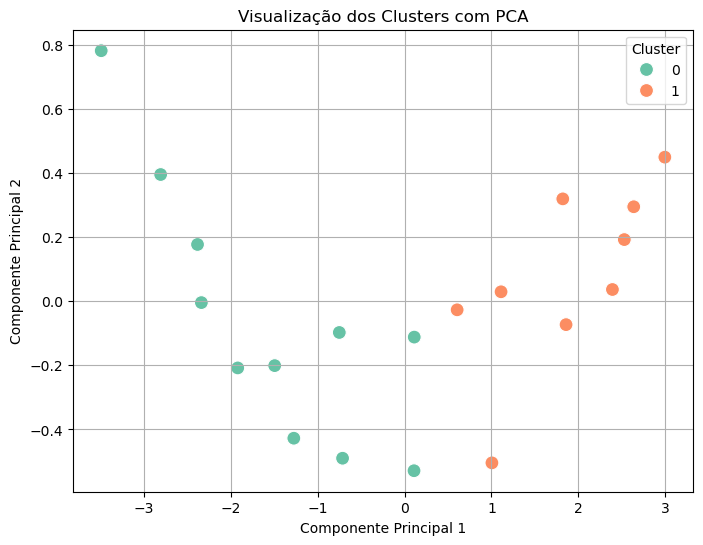
\includegraphics[keepaspectratio]{teste_quarto_files/figure-pdf/cell-15-output-1.png}}

\begin{Shaded}
\begin{Highlighting}[]
\CommentTok{\# Parte 9: Interpretação dos Perfis}
\BuiltInTok{print}\NormalTok{(}\StringTok{"}\CharTok{\textbackslash{}n}\StringTok{Médias por cluster:"}\NormalTok{)}
\NormalTok{df.groupby(}\StringTok{\textquotesingle{}cluster\textquotesingle{}}\NormalTok{)[features].mean().}\BuiltInTok{round}\NormalTok{(}\DecValTok{2}\NormalTok{)}
\end{Highlighting}
\end{Shaded}

\begin{verbatim}

Médias por cluster:
\end{verbatim}

\begin{longtable}[]{@{}lllll@{}}
\toprule\noalign{}
& acessos & participacoes & entregas & nota\_final \\
cluster & & & & \\
\midrule\noalign{}
\endhead
\bottomrule\noalign{}
\endlastfoot
0 & 11.55 & 3.91 & 0.53 & 5.23 \\
1 & 37.22 & 16.11 & 0.93 & 8.89 \\
\end{longtable}




\end{document}
